% Progress presentation, 17/11 -> 23/11/2026 (experiment 0014, partial; paper in the ACL template).
% Tables: poetry run python scripts/make_presentation_0014_tables.py
%   cd presentation && latexmk -pdf avancos_2026-11-23.tex
\documentclass[aspectratio=169,10pt]{beamer}
\usepackage[T1]{fontenc}
\usepackage[utf8]{inputenc}
\usepackage[brazil]{babel}
\usepackage{booktabs,multirow,array,graphicx,amsmath,bm}
\usepackage{xcolor}
\usepackage{tikz}
% Shared macros. Change \model once to rename the architecture everywhere.
\newcommand{\model}{COVER}
\newcommand{\todo}[1]{\textcolor{red}{[TODO: #1]}}

% Labels and sets
\newcommand{\E}{\textsc{e}}
\newcommand{\N}{\textsc{n}}
\newcommand{\C}{\textsc{c}}
\newcommand{\Prem}{\mathcal{P}}
\newcommand{\Hyp}{\mathcal{H}}
\newcommand{\Rel}{\mathcal{R}}
\newcommand{\Ops}{\mathcal{O}}
\newcommand{\cls}{\textsc{[cls]}}
\newcommand{\nullnode}{\varnothing}
\newcommand{\Lset}{\mathcal{L}_{\mathrm{set}}}
\newcommand{\Pcov}{P_{\mathrm{cov}}}
\newcommand{\Pnc}{P_{\neg\mathrm{conf}}}
\newcommand{\LN}{\operatorname{LN}}
\newcommand{\MLP}{\operatorname{MLP}}
\newcommand{\softplus}{\operatorname{softplus}}
\newcommand{\vect}[1]{\bm{#1}}
\providecommand{\best}[1]{\textbf{#1}}  % best value of a column in the result tables (boxed in the slides)

\renewcommand{\todo}[1]{}
\renewcommand{\cls}{[CLS]}
\usepackage{amssymb}
% best value of each column in the result tables: bold with a red box
\renewcommand{\best}[1]{{\setlength{\fboxsep}{0.8pt}\setlength{\fboxrule}{0.7pt}\fcolorbox{red}{white}{\textbf{#1}}}}

\definecolor{neural}{HTML}{2F6DB5}
\definecolor{symb}{HTML}{D9822B}
\definecolor{logic}{HTML}{2E8B57}
\definecolor{relneg}{HTML}{C0392B}

\usetheme{default}
\setbeamercolor{background canvas}{bg=white}
\setbeamercolor{frametitle}{fg=black}
\setbeamercolor{title}{fg=black}
\setbeamercolor{structure}{fg=neural}
\setbeamerfont{frametitle}{series=\bfseries,size=\large}
\setbeamertemplate{navigation symbols}{}
\setbeamertemplate{itemize items}[circle]
\setbeamertemplate{footline}{\hfill\textcolor{black!45}{\scriptsize\insertframenumber/\inserttotalframenumber}\hspace{1em}\vspace{0.6em}}

\newcommand{\up}[1]{\textcolor{logic}{\textbf{#1}}}
\newcommand{\down}[1]{\textcolor{relneg}{\textbf{#1}}}
\newcommand{\take}[1]{\vspace{4pt}\begin{beamercolorbox}[sep=5pt,rounded=true]{take}\small #1\end{beamercolorbox}}
\setbeamercolor{take}{bg=black!5,fg=black}
\newcommand{\tab}[2][1]{\resizebox{#1\linewidth}{!}{\input{tables_0014/#2}}}
\newcommand{\done}{\textcolor{logic}{\textbf{completo}}}
\newcommand{\running}{\textcolor{symb}{\textbf{rodando}}}
\newcommand{\queued}{\textcolor{black!50}{na fila}}

\title{Experimentos em Natural Language Inference (NLI)}
\author{}
\date{23 de novembro de 2026}

\begin{document}

\begin{frame}[plain]
  \centering\vfill
  {\fontsize{30}{36}\selectfont\bfseries Experimentos em\\[4pt] Natural Language Inference (NLI)\par}
  \vspace{1.2cm}
  {\large 23 de novembro de 2026\par}
  \vfill
\end{frame}

% --------------------------------------------------------------------------
\begin{frame}{O que aconteceu desde 17/11}
\begin{enumerate}\setlength{\itemsep}{6pt}
\item \textbf{Experimento 0014} provisionado e rodando nas duas máquinas: replica o 0011 com \textbf{encoders grandes}.
  \begin{itemize}\small
  \item Português: \textbf{Albertina-900M} (sugestão do survey de modelos para o português).
  \item Entre línguas: \textbf{XLM-R-large} no lugar do XLM-R-base.
  \item Ablação de \textbf{cada léxico separado} (inglês, português e entre línguas).
  \end{itemize}
\item \textbf{Resultados parciais:} 166 de 380 runs prontos.
\item \textbf{Artigo} adaptado ao template do \textbf{ACL 2027} (submissão via ARR).
\end{enumerate}
\end{frame}

% --------------------------------------------------------------------------
\begin{frame}{Experimento 0014: o que está rodando}
\centering\small
\resizebox{\linewidth}{!}{\begin{tabular}{@{}llllrl@{}}
\toprule
Bloco & Encoder & Treino & O que compara & Runs & Status \\
\midrule
Ablação de léxicos & RoBERTa-large & SICK & só WordNet / só Wikt. & 20 & \done{} \\
Ablação PT & Albertina-900M & InferBR & 7 variantes (como no 0011) & 70 & \running{} (53) \\
Léxicos PT & Albertina-900M & InferBR & só PT-LKB / só Wikt. & 20 & \queued{} \\
Baselines de grafo PT & Albertina-900M & InferBR & K-BERT, KGAnet, KGNLI & 30 & \queued{} \\
\midrule
Ablação EN$\to$PT & XLM-R-large & SICK & 7 variantes & 70 & \done{} \\
Ablação PT$\to$EN & XLM-R-large & InferBR & 7 variantes & 70 & \running{} (23) \\
Baselines de grafo XL & XLM-R-large & ambos & K-BERT, KGAnet, KGNLI & 60 & \queued{} \\
Léxicos XL & XLM-R-large & ambos & $-$ Wikt. / $-$ WordNet e PT-LKB & 40 & \queued{} \\
\bottomrule
\end{tabular}}\\[8pt]
\raggedright\footnotesize
\begin{itemize}\setlength{\itemsep}{2pt}
\item Mesmo protocolo do 0011: 10 seeds por sistema, pareado por seed, mesmos conjuntos de teste e mesma métrica (MCC).
\item Previsão: máquina A (inglês e XLM-R) $\sim$30/11; máquina B (Albertina) $\sim$5/12.
\end{itemize}
\end{frame}


% --------------------------------------------------------------------------
\begin{frame}{Léxicos: quanto cada um cobre}
\textit{\small \% de pares de treino com pelo menos uma relação entre uma palavra da hipótese e uma da premissa}\\[6pt]
\begin{columns}[T]
\column{0.5\textwidth}
\centering\small
\textbf{SICK (inglês)}\\[3pt]
\begin{tabular}{@{}lrr@{}}
\toprule
Léxico & Pares & Antônimos \\
\midrule
WordNet & 49,3\% & 538 \\
Wiktionary & 19,2\% & 232 \\
\midrule
WordNet + Wikt.\ (modelo) & \textbf{52,1\%} & \textbf{611} \\
\bottomrule
\end{tabular}
\column{0.5\textwidth}
\centering\small
\textbf{InferBR (português)}\\[3pt]
\begin{tabular}{@{}lrr@{}}
\toprule
Léxico & Pares & Antônimos \\
\midrule
PT-LKB & 46,7\% & 0 \\
Wiktionary & 5,4\% & 316 \\
\midrule
PT-LKB + Wikt.\ (modelo) & \textbf{48,2\%} & \textbf{316} \\
\bottomrule
\end{tabular}
\end{columns}
\take{No inglês o \textbf{WordNet faz quase tudo}: o Wiktionary acrescenta só +2,8 de cobertura. No português o \textbf{PT-LKB faz quase tudo}, mas não tem nenhum antônimo: eles vêm só do Wiktionary.}
\end{frame}

% --------------------------------------------------------------------------
\begin{frame}{Inglês: qual léxico importa? (RoBERTa-large, MCC)}
\textit{\small Treino no SICK; cada linha é o \model{} com um léxico diferente} \hfill {\scriptsize $^\dagger$ $p<.05$ contra o [CLS]}\\[3pt]
\centering\tab[0.92]{lex_en}
\take{\textbf{O léxico quase não importa.} Com qualquer um deles o \model{} ganha do [CLS] fora da distribuição (AX-b \up{+4.7 a +5.3}, ConjNLI \up{+4.5 a +5.9}, FraCaS \up{+8.6 a +10.0}, todos $p<.05$), e as diferenças entre léxicos ficam dentro do desvio entre seeds. Até o Wiktionary, que cobre só 19\% dos pares, basta. O ganho vem da \textbf{estrutura} (cobertura), não da quantidade de conhecimento.}
\end{frame}

% --------------------------------------------------------------------------
\begin{frame}{Português: Albertina-900M (MCC)}
\textit{\small Treino no InferBR} \hfill {\scriptsize $^\dagger$ $p<.05$ contra o Albertina [CLS]}\\[3pt]
\centering\tab[0.85]{pt_large}
\take{\textbf{Encoder maior ajuda muito:} o [CLS] sobe de 4 a 10 pontos. \textbf{O \model{} continua ajudando} em cima dele: \up{+2.3} no ASSIN\,2 e \up{+2.3} no SICK-BR ($p<.05$), e \textbf{metade do desvio entre seeds} (ASSIN $\pm$5.9$\to\pm$3.5; SICK-BR $\pm$2.4$\to\pm$1.2). Destaque: o BERTimbau-base + \model{} (110M) \textbf{empata com o Albertina [CLS] (900M)} no ASSIN\,2 e no SICK-BR.}
\end{frame}


% --------------------------------------------------------------------------
\begin{frame}{Entre línguas EN$\to$PT com XLM-R-large (MCC)}
\textit{\small Treino no SICK (inglês), sem nenhum exemplo em português} \hfill {\scriptsize $^\dagger$ $p<.05$ contra o XLM-R-large [CLS]}\\[3pt]
\centering\tab[0.85]{xl_large_pt}
\take{\textbf{Na transferência para o português o \model{} perde:} InferBR \down{$-$3.3} e ASSIN \down{$-$4.1} ($p<.05$); empata no ASSIN\,2 e no SICK-BR. Com o XLM-R-base (0011) era empate. Vai para as \textbf{limitações} do artigo.}
\end{frame}

% --------------------------------------------------------------------------
\begin{frame}{Entre línguas PT$\to$EN com XLM-R-large (MCC)}
\textit{\small Treino no InferBR (português), sem nenhum exemplo em inglês} \hfill {\scriptsize $^\dagger$ $p<.05$ contra o XLM-R-large [CLS]}\\[3pt]
\centering\tab[0.85]{xl_large_pt_to_en}
\take{\textbf{Nesta direção o \model{} ainda ajuda, mas menos:} empata no SICK, ganha no ConjNLI \up{+3.4} ($p<.05$), AX-b \up{+2.0} e FraCaS \up{+0.9} (n.s.), e perde no Breaking NLI \down{$-$6.0} ($p<.05$), como no EN$\to$PT. Com o XLM-R-base (0011) o ganho era maior: SICK \up{+4.7} e ConjNLI \up{+6.3} ($p<.05$). O ganho da estrutura diminui com o encoder grande.}
\end{frame}

% --------------------------------------------------------------------------
\begin{frame}{Artigo no template do ACL 2027}
\begin{columns}[c]
\column{0.42\textwidth}
\centering
\fbox{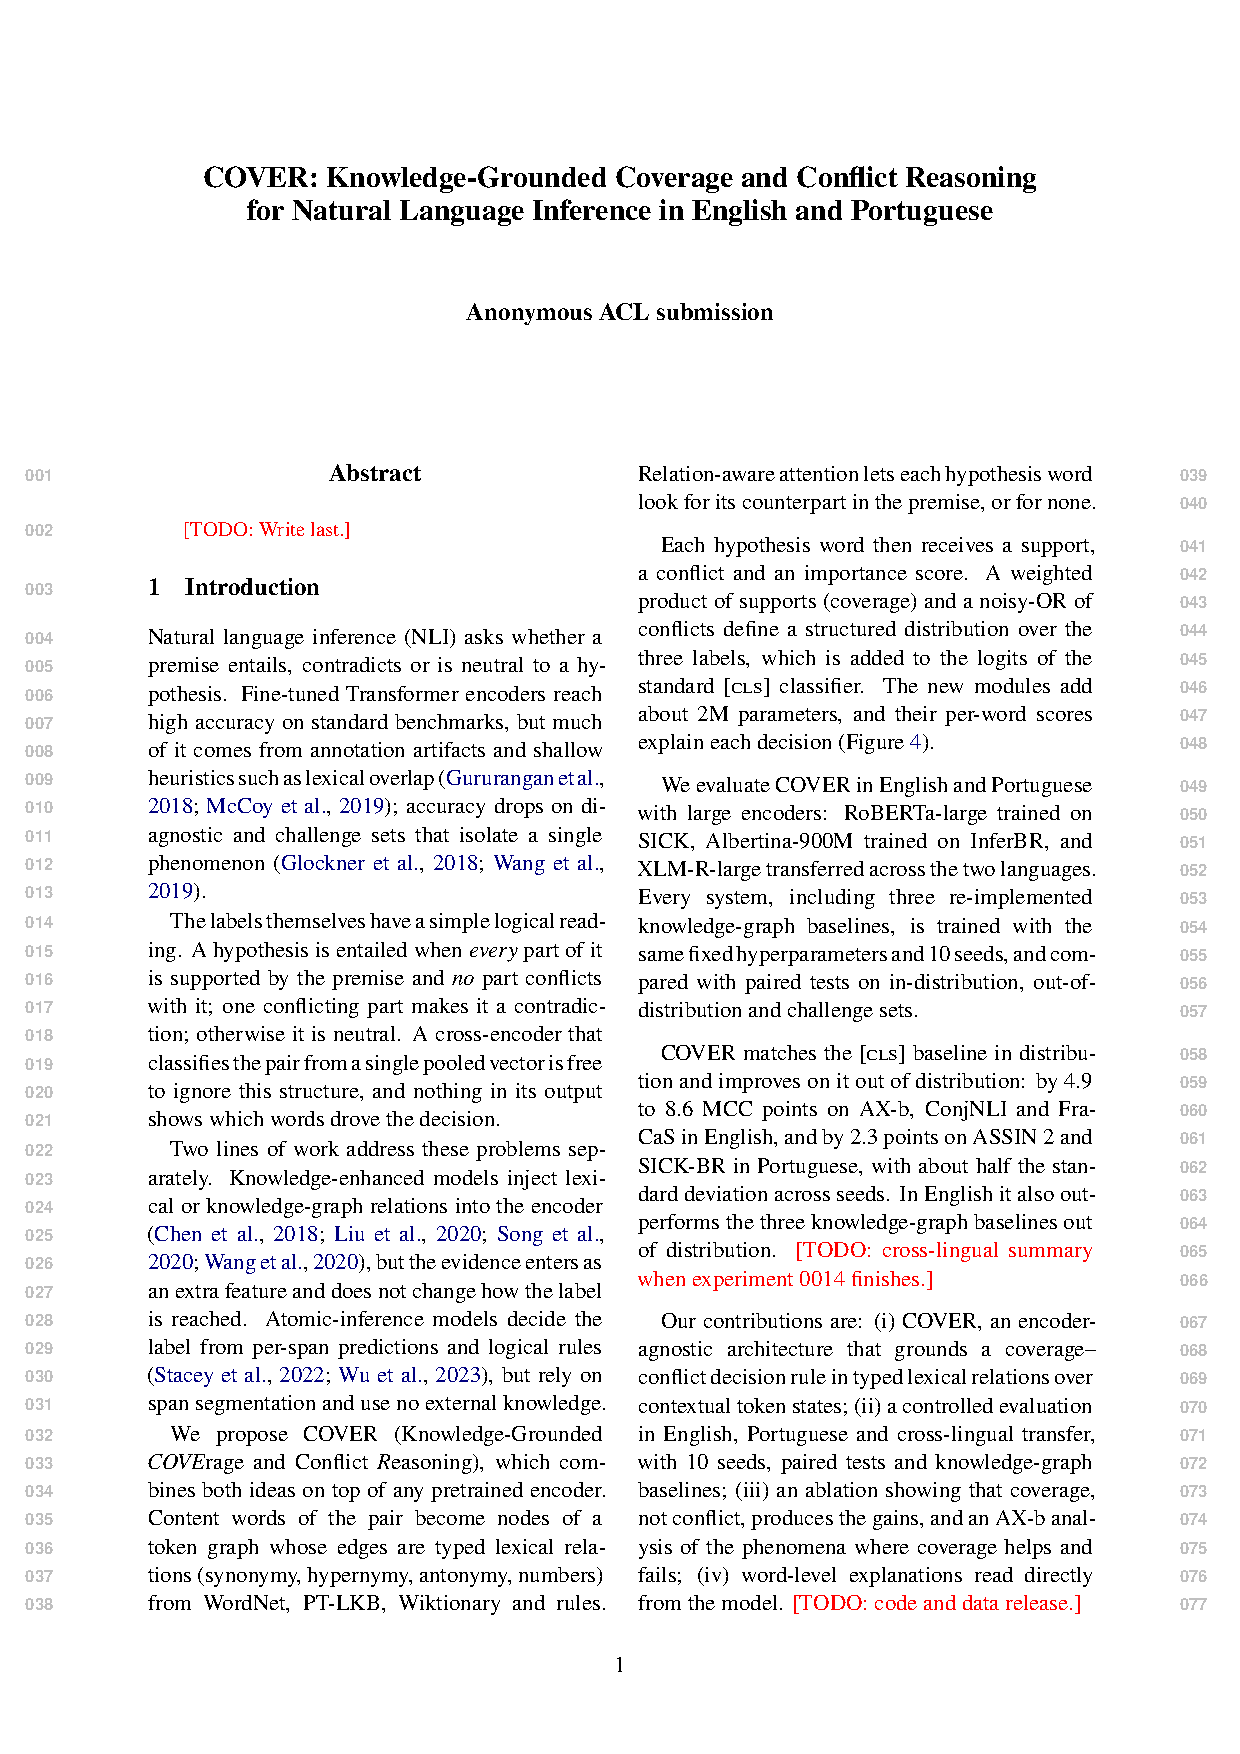
\includegraphics[page=1,width=0.44\linewidth]{../paper/main.pdf}}\hspace{2pt}%
\fbox{\includegraphics[page=3,width=0.44\linewidth]{../paper/main.pdf}}
\column{0.55\textwidth}
\footnotesize
\textbf{Feito}
\begin{itemize}\setlength{\itemsep}{2pt}
\item Estilo oficial do ACL (\texttt{acl.sty}) em modo revisão: anônimo e com linhas numeradas.
\item Referências no estilo ACL; seção \textbf{Limitations} criada (obrigatória).
\item Tabelas e equações ajustadas à coluna mais estreita.
\end{itemize}
\textbf{Regras da submissão (ARR)}
\begin{itemize}\setlength{\itemsep}{2pt}
\item Prazo: \textbf{4 de janeiro de 2027}.
\item Artigo longo: \textbf{8 páginas} (+1 na versão final); limitações, referências e apêndices não contam.
\item Checklist de pesquisa responsável preenchido no envio.
\end{itemize}
\textbf{Problema:} o corpo hoje ocupa $\sim$10 páginas. As páginas 8--10 são só tabelas: mover parte para o apêndice.
\end{columns}
\end{frame}

% --------------------------------------------------------------------------
\begin{frame}{Conclusões parciais do 0014}
\small
\begin{enumerate}\setlength{\itemsep}{5pt}
\item \textbf{O padrão do 0011 se mantém com encoders grandes:} o \model{} empata in-distribution e ganha fora dela (RoBERTa-large e Albertina-900M).
\item \textbf{O léxico importa pouco no inglês:} qualquer dicionário dá o mesmo ganho.
\item \textbf{Albertina:} o ganho do \model{} diminui com o encoder grande, mas continua significativo em 2 de 4 testes, e a variância cai pela metade.
\item \textbf{Ponto fraco:} transferência com XLM-R-large; EN$\to$PT perde no InferBR e no ASSIN, PT$\to$EN só ganha no ConjNLI.
\end{enumerate}
\end{frame}

% --------------------------------------------------------------------------
\begin{frame}{Próximos passos}
\small
\begin{itemize}\setlength{\itemsep}{5pt}
\item Terminar o 0014: ablação completa do Albertina, léxicos PT, PT$\to$EN e baselines de grafo com encoders grandes.
\item Artigo: escrever resultados e discussão; cortar para 8 páginas; escrever as limitações.
\item Atualizar as tabelas do artigo com os encoders grandes quando o 0014 terminar.
\end{itemize}
\end{frame}

\end{document}
